\chapter{Theory}

\section{The transmon qubit}
The qubit under investigation during this project is the so called transmon qubit. A traditional transmon qubit consists of a pair of Josephson junctions connected to two superconducting pads. The structure is surrounded by a grounded metal plane. Other parts of the structure are the readout resonator, the coupling resonator, the flux control, and the feedline. They are Co-Planar Waveguides (CPW) enabling readout, coupling to other qubits, and frequency control. These parts will not be considered during simulation of the qubits and therefore not described in detail here. An overview of a transmon qubit can be found in figure \ref{fig:transmonblueprint} \cite{Riste2014}.

\begin{figure}
	\begin{center}
		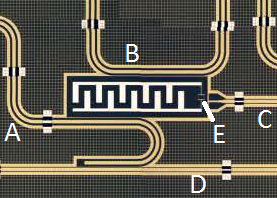
\includegraphics[scale=1]{Figures/Transmon/transmonblueprint_zoomed2}
		\caption{An overview of the transmon qubit with two superconducting pads in the centre. The qubit is connected to several structures: the readout resonator (A), the coupling resonator (B), the flux control (C), and the feedline (D). The location of the Josephson junction (E) is also indicated.}
		\label{fig:transmonblueprint}
	\end{center}
\end{figure}

\begin{figure}
	\begin{center}
		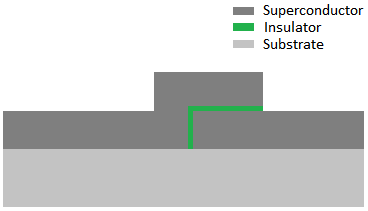
\includegraphics[scale=1]{Figures/Transmon/JJ}
		\caption{The Josephson junction. Two superconducting electrodes (Al) separated by an insulator (AlOx) on a substrate (Si)}
		\label{fig:JJ}
	\end{center}
\end{figure}

A Josephson junction consists of two layers of superconducting material separated by an insulating layer. A simple representation of the Josephson junction can be found in figure \ref{fig:JJ}. It behaves like a non-linear inductor \cite{You2011}.
The transmon qubit can therefore be treated as a simple LC-circuit. The Josephson junction is replaced by an inductor and the different capacitances are replaced by an single equivalent capacitor. The resulting simplified system can be seen in figure~\ref{fig:LCcircuit}. The energy in an LC-circuit is stored in the electric field of the capacitor and the magnetic field of the inductor. As the circuit resonates the energy is moved between the two with a certain frequency.
This resonance frequency is given by formula \eqref{eq:ResonanceFrequency} below.

\begin{equation} \label{eq:ResonanceFrequency}
f_{0}=\frac{1}{2\pi\sqrt{LC}}
\end{equation}
Where \(L\) is the inductance and \(C\) is the capacitance. Specific resonance frequencies can be targeted by changing the qubit's design.

\begin{figure}
	\begin{center}
		\begin{circuitikz}
			\draw (0,0)
			to[open,*-,v=$U_q$] (0,2) % The voltage source
			to[short,*-] (2,2)
			to[L=$L_1$] (2,0) % The inductor
			to[short] (0,0);
			\draw (2,2)
			to[short] (4,2)
			to[C=$C_1$] (4,0)
			to[short] (2,0);
		\end{circuitikz}
		\caption{A simple parallel LC-circuit}
		\label{fig:LCcircuit}
		\end{center}
\end{figure}

\subsection{Energy in an LC-circuit}
In order to determine the participation ratio of the lossy layers in storing energy in the system, the total energy must be know. The total energy stored in an LC-circuit at any time can be calculated as follows:
\begin{equation} \label{eq:totalenergy}
W_{tot}=\frac{1}{2}CV_{max}^{2}
\end{equation}
Where \(C\) is the total capacitance of the system and \(V_{max}\) the maximum voltage over capacitor. Both the capacitance and the voltage will be retrieved from the simulation.



\section{Electric fields}
Of specific interest is the manner in which the circuit's energy is stored in its electric field. The distribution of the field determines where the energy is stored. This distribution will be retrieved via simulation. 

\subsection{Boundary conditions}
When the electric field crosses an interface between two materials having different dielectric constants the strength of the field is altered. While the tangential component remains equal across the interface, for the normal component it is the product of the dielectric constant and the electric field that is constant. So:

\begin{subequations}\label{eq:ContinuityEq}
	\begin{equation} \label{eq:ContinuityEqA}
	E_{1}^{\parallel} = E_{2}^{\parallel}
	\end{equation}	
	\begin{equation} \label{eq:ContinuityEqB}
	\epsilon_{1}E_{1}^{\bot} = \epsilon_{2}E_{2}^{\bot}
	\end{equation}
\end{subequations}

These equations are only valid when there is no free charge of free current at the interface.
Furthermore, it is approximated that the electric field on the surface of the metal is purely perpendicular.
\subsection{Stored energy}
The energy stored in the electric field in a material can be calculated using equation \eqref{eq:energy} below.
\begin{equation} \label{eq:energy}
W = \frac{\epsilon}{2}\int{|E|}^{2}dV
\end{equation}
Where \(\epsilon\) is the permittivity of the material and \(V\) is the volume occupied by the material. 

\section{Sources of decoherence}
In order for the qubit to be coherent for a sufficiently long time period, sources of decoherence must be eliminated. Sources include spontaneous emission, the Purcell Effect, quasiparticle tunnelling and flux coupling \cite{Koch2007}.  \todo{Explaination necessary?} 
The source in question during this project is the loss through dielectric materials in the system. It is believed to be a prominent, if not limiting source of decoherence \cite{Koch2007}\cite{PhysRevLett.95.210503}. 
 
\subsection{Perfect Electric Conductor}
As the qubit is supercooled to a temperature of only 10 mK, the metal in the qubit is treated as a Perfect Electric Conductor (PEC). As the LC-circuit resonates, this means the flowing current wont dissipate any energy through resistance. 
 
\subsection{Dielectric loss}
During production of qubits, different procedures introduce lossy materials to the structure. An important property of each of these materials is their permittivity. It will determine the strength of the field and the energy stored inside the layers (see formula \eqref{eq:energy}). Different layers on distinct material interfaces created during certain production steps can have different dielectric constants.   
Impurities existing in these layers are so called two-level systems. The coupling of the qubit to these two-level systems is the source of decoherence of interest during this research. 

\section{The participation ratio}
To determine what kind of structure design may improve coherence time the participation ratio of lossy layers can be calculated. If the assumption is made that the electric field remains constant inside the lossy layer, equation~\eqref{eq:energy} can be rewritten as follows:
\begin{equation}\label{eq:energy_layer}
W = \frac{\epsilon}{2}t\int{|E|}^{2}dA
\end{equation}
Where \(\epsilon\) is the permittivity of the material and \(t\) is the thickness of the lossy layer. Furthermore, \(A\) is the surface area of the lossy layer. By comparing the energy stored in each individual layer to the total energy in the LC-circuit the participation ratios can be calculated:

\begin{equation}\label{eq:PartRatio}
p_{\textit{i}}=\frac{W_{\textit{i}}}{W_{tot}}
\end{equation}


